\documentclass[11pt]{article}
\usepackage[T1]{fontenc}
\usepackage{lmodern,microtype,amsmath,amssymb,amsthm}
\usepackage[hmargin=1in,top=0.86in,bottom=0.88in]{geometry}
\usepackage{xcolor}
\definecolor{linkblue}{HTML}{1558B0}
\usepackage{tikz}
\usepackage[font=small,labelfont=bf,labelsep=period]{caption}
\usepackage[colorlinks=true,allcolors=linkblue,pdfauthor={twinheterodox},pdftitle={Smooth convergents and the size of the next denominator}]{hyperref}
\usepackage{enumitem}
\newtheorem{theorem}{Theorem}[section]
\newtheorem{lemma}[theorem]{Lemma}
\newtheorem{corollary}[theorem]{Corollary}
\newcommand{\M}{\mathcal M}
\newcommand{\R}{\mathbb R}
\newcommand{\Z}{\mathbb Z}
\newcommand{\sgnunit}{\{\pm1\}}
\title{Smooth convergents and the size of the next denominator}
\author{twinheterodox\\[-1pt]{\small Prepared with Codex}}
\date{November 24, 2026}
\linespread{0.985}
\begin{document}
\maketitle
\vspace{-1.5\baselineskip}
\begin{abstract}
Suppose an irrational $\xi$ has infinitely many continued-fraction convergents
$P/q$ for which $|P|$, $q$, and the next denominator $Q$ have all their prime
factors in a fixed finite set $S$. Marques proved that $\log Q\gg q^c$ at
those indices for some $c>0$. When $S$ consists of two primes, the bound
holds with $c=1$, which is sharp. When $S$ consists of three primes, the
supremal exponent is at most $1/2$. In every fixed open subinterval of
$(1,2)$, the minimum of $\log Q$ over $\xi$ and $P/q$ in the interval
has order $\sqrt q$ at infinitely many powers $q$ of each prime in $S$.
Let $N_q$ be the least $S$-smooth integer greater than $1$ congruent to
$\pm1\pmod q$. For each $S$ with at least three primes, a
single irrational realizes $P Q=N_q$ infinitely often.
\end{abstract}
\vspace{-0.6\baselineskip}

\section{The size of the next denominator}
Let $p_n/q_n$ be the regular continued-fraction convergents of a real
irrational $\xi$, and fix a finite set $S$ of primes. In 1939 Erd\H{o}s
and Mahler proved that if $q_{n-1},q_n,q_{n+1}$ all have their prime
factors in $S$ for infinitely many $n$, then $\xi$ is a Liouville number
(its irrationality exponent is infinite). They also considered the primes
dividing $|p_n|q_n$. If these all lie in $S$ for infinitely many $n$,
they observed that $\xi$ must be transcendental and asked whether it
must be Liouville \cite[pp.~17--18]{em}.

In 2017 Lelis and Marques proved the conjecture under a spacing hypothesis
on the selected indices \cite[Theorem~1.1]{lm}. Bugeaud and Nguyen still
listed the general case as open in 2023 \cite[Question~4.1]{bn}. In a
November 2026 preprint Marques disproved the conjecture by constructing a
number of irrationality exponent $4$ with infinitely many convergents of
the form $2^a/3^b$ \cite{counter}.

In an August 2026 paper Marques also imposed the prime restriction on the
immediate next denominator. Write $P/q=p_n/q_n$ and $P'/Q=p_{n+1}/q_{n+1}$.
Call the transition
\emph{$S$-smooth} if all prime factors of $|P|,q,Q$ belong to $S$.
Marques proved that infinitely many such transitions force
$\log Q\gg_{\xi,S}q^{c(S)}$ at those indices for an
effective $c(S)>0$ \cite[Theorem~1.1]{marques}. Since the error in $P/q$
lies between $1/[q(Q+q)]$ and $1/(qQ)$, this bound forces $\xi$ to be
Liouville.

How large can the exponent in Marques's bound be? Let $c_*(S)$ be the
supremum of the $c\ge0$ for which every such $\xi$ satisfies $\log Q\gg_{\xi,S,c}q^c$
along its $S$-smooth transitions. We prove $c_*(S)=1$ when $S$ consists
of two primes and $c_*(S)\le\tfrac12$ when $S$ consists of three.
In the two-prime case, $q$ and $|P|Q$ are coprime, so each uses a different
prime. The linear bound holds, and one irrational attains $\log Q\asymp q$
infinitely often. With three primes, a denominator using two primes still
gives a linear bound. With $\xi$ and $P/q$ in any fixed open subinterval
of $(1,2)$, the minimum of $\log Q$ has order $\sqrt q$ at infinitely many
powers $q=\ell^v$ of each denominator prime $\ell$.
Minima below $q^{1/2-\epsilon}$ at infinitely many other powers, for some
fixed $\epsilon>0$, would lower the exponent further. Corollary~\ref{cor:support}
identifies $c_*(S)$ with the least of the three lower-limit exponents.

Among continued fractions having $P/q=65{,}536/59{,}049=2^{16}/3^{10}$
as a convergent, how small can the next denominator be? If $Q$ is a power
of $2$, its least possible value has $5{,}921$ decimal digits. Allow $5$
as well and the minimum has just $19$ digits. Section~\ref{sec:exact}
computes both minima.

To study one denominator prime, fix $\ell$ and a nonempty finite set $R$
of other primes. Write $\M(R)$ for the positive integers supported on
$R$, including $1$. Take $q=\ell^v>2$ and $P,Q\in\M(R)$. The determinant
$|P'q-P Q|=1$ gives $P Q\ge N_q$, where $N_q$ is the least integer $>1$
in $\M(R)$ congruent to $\pm1$ modulo $q$. For each nonempty open
interval $I\subset(1,2)$, let $T_v(I)$ be the minimum of $\log Q$ as
the irrational $\xi$ and its convergent $P/q$ both vary in $I$. An
empty minimum has value $+\infty$. All logarithms are natural.

The implied constant in Marques's bound can depend on $\xi$, so sharpness
requires infinitely many small successors in one continued fraction. A
finite prefix specifies an interval of possible irrational continuations.
Constructing the next transition inside that interval preserves the prefix
and every transition already chosen.

\begin{theorem}\label{th:scales}
The following hold, with positive constants $c,C$ depending only on
$\ell$ and $R$.
\begin{enumerate}[label=(\roman*),nosep]
\item If $R=\{r\}$, every admissible pair with $P/q\in(1,2)$ satisfies
$\log Q\ge cq$ for all large $v$. In every $I$, infinitely many $v$
also satisfy $T_v(I)\le Cq$.
\item If $R=\{r,s\}$, there is an infinite set $V$ of levels depending
only on the primes such that for every $I$ and all sufficiently large
$v\in V$,
\[
                       c\sqrt q\ \le\ T_v(I)\ \le\ C\sqrt q .
\]
The lower bound applies to every admissible pair at these levels with
$P/q\in(1,2)$.
\end{enumerate}
For each choice of primes there is a dense $G_\delta$ subset of the
irrationals in $(1,2)$ whose continued fractions attain the indicated
two-sided bounds at infinitely many indices.
\end{theorem}

For $|R|\ge2$, Theorem~\ref{th:transfer} gives $T_v(I)\asymp_I\log N_q$
at every sufficiently large power, with the primes fixed. To attain
$P Q=N_q$ repeatedly in one continued fraction, the minimizing product at
each chosen power must have a divisor $P$ for which $P/q$ extends the
prefix already chosen. Theorem~\ref{th:exact} finds such divisors along
powers where $\log\log N_q/\log q$ tends to its lower limit.
For $q=3^v$ and $R=\{2,5\}$, it remains open whether one irrational
can attain $\log Q\le q^{1/2-\epsilon}$ at infinitely many powers outside
$V$ for some fixed $\epsilon>0$.

\paragraph{Precedents.}
Erd\H{o}s and Mahler also observed that all the convergent denominators
of one irrational can be supported on two prescribed primes
\cite[p.~18]{em}. Adiceam gives a
recursion making successive denominators alternate between prime powers
\cite[proof of Theorem 2, preprint version]{adiceam}. The numerator at the selected index
is unrestricted in that construction. Bugeaud and Nguyen prescribe prime
supports at selected rational approximants \cite[\S4]{bn}. If
$n_1<n_2<\cdots$ are the selected indices, Lelis and Marques bound the
denominator $q_{n_{j+1}}$ at the next selected index \cite[(2.1)]{lm}.
Here $Q=q_{n_j+1}$ follows $q_{n_j}$ immediately.
For the $2^a/3^b$ convergents in Marques's counterexample, the largest
prime factor of $Q$ must tend to infinity by his neighboring-denominator
theorem \cite[Theorem~1.1]{marques}. Marques already constructs infinitely many
pairs with $(P,q,Q)=(2^u,3^v,2^w)$ \cite[p.~2]{marques}.
The rank-one estimate below quantifies this construction. For two auxiliary
primes the main additional ingredient is the geometry of planar
$\ell$-adic approximation lattices, as in de Weger \cite{dw}.

\section{From a congruence to consecutive convergents}
\begin{lemma}\label{lem:cyl}
Let $P/q\in(1,2)$ be reduced, with $q>2$, and let $Q>q$ be an integer.
There exists an irrational whose continued fraction has $P/q$ as a
convergent and $Q$ as its next denominator if and only if
$P Q\equiv\pm1\pmod q$. In that case the
irrational numbers with a suitable finite prefix form the irrational
points of an open interval within distance $1/(qQ)$ of $P/q$.
\end{lemma}
\begin{proof}
Necessity follows from $|P' q-P Q|=1$. Take the finite expansion of
$P/q$ whose last partial quotient is at least $2$, and also the expansion
obtained by splitting that quotient as $a=(a-1)+1/1$. If the preceding
denominator for the first expansion is $h$, that for the second is $q-h$.
They give the two residues $\pm P^{-1}\pmod q$ by the determinant
identity. Choose the expansion with preceding denominator $h'$ congruent
to $Q$, and append the positive partial quotient $(Q-h')/q$.
The recurrence gives a next convergent $P'/Q$. As the remaining complete
quotient ranges over the irrationals greater than $1$, the endpoints of
the resulting cylinder are $P'/Q$ and $(P'+P)/(Q+q)$. Their distances
from $P/q$ are $1/(qQ)$ and $1/(q(Q+q))$, respectively.
\end{proof}

For example, $4\cdot5\equiv-1\pmod3$. The convergent $4/3=[1;2,1]$
has preceding denominator $2$. Appending $(5-2)/3=1$ gives $7/5$ as
the immediate successor. Section~\ref{sec:exact} exhibits a second
smooth pair inside this same cylinder.

\begin{lemma}\label{lem:unit}
For a fixed positive rational $\ell$-adic unit $z\ne1$, if $m\ge1$ and
$z^m\equiv\pm1\pmod{\ell^v}$, then $m\gg_{\ell,z}\ell^v$.
\end{lemma}
\begin{proof}
Put $h=2(\ell-1)$ and $e=\operatorname{ord}_\ell(z^h-1)$. Here $e\ge1$,
and $e\ge3$ when $\ell=2$ since an odd unit squares to $1$ modulo $8$.
By the binomial expansion, raising $1+\ell^e u$, with $u$ a unit, to an
exponent prime to $\ell$ preserves the valuation of its difference from $1$.
Raising it to $\ell$ increases that valuation by one. Hence
$\operatorname{ord}_\ell(z^{hm}-1)=e+\operatorname{ord}_\ell(m)$.
Since $h$ is even, $v\le e+\operatorname{ord}_\ell(m)$.
\end{proof}

If $R=\{r\}$, write $P Q=r^b$. Lemmas~\ref{lem:cyl} and~\ref{lem:unit}
give $b\gg q$, and $\log P\le\log(2q)$ gives the lower bound in
Theorem~\ref{th:scales}(i). For the converse let $J$ be an open interval
whose closure lies inside $I$. Infinitely many $v$ admit $u\ge0$ with
$r^u/\ell^v\in J$, by the irrationality of $\log\ell/\log r$ and density
of the tails of an irrational rotation. The least $b>0$ with
$r^b\equiv\pm1\pmod q$ lies between $c_0q$ and $\varphi(q)$. For large
such $v$ take $P=r^u$, $Q=r^{b-u}>q$. Lemma~\ref{lem:cyl} gives an
entire cylinder in $I$ with $\log Q\le q\log r$.

For two distinct primes $r,s$ we will use a stronger elementary
observation. For \emph{every} sufficiently large real $y$, a fixed such
interval $J$ contains $r^u s^w/y$ with $u,w\ge0$ and $w\le M_J$.
To see this, shrink $J=(a,b)$ so that $\log(b/a)<\log r$.
The positive multiples of $\log s$ are dense modulo $\log r$, so a
fixed finite initial segment meets every translate of the open arc of
length $\log(b/a)$. Hence some $w\le M_J$ and integer $u$ satisfy
$\log(ay)<u\log r+w\log s<\log(by)$. Boundedness of $w$ gives $u\ge0$
for large $y$.

\section{Powers with a square-root minimum}
For $R=\{r,s\}$ let
\[
 \Lambda_v=\{(a,b)\in\Z^2:r^a s^b\equiv\pm1\pmod{\ell^v}\}.
\]
Negative powers are defined using modular inverses. The index $D_v$ of
$\Lambda_v$ is the order of the subgroup generated by $r,s$ in
$(\Z/q\Z)^\times/\sgnunit$. The order of $r$ alone is $\gg q$ by
Lemma~\ref{lem:unit}, so $D_v\asymp q$. Successive lattices satisfy
$\Lambda_v\subseteq\Lambda_{v-1}$ and
$\ell\Lambda_{v-1}\subseteq\Lambda_v$ for $v\ge2$. The second follows
by raising the defining congruence to the $\ell$th power.

\begin{lemma}\label{lem:balanced}
There are infinitely many $v$ at which the length of the shortest
nonzero vector of $\Lambda_v$ is $\gg\sqrt q$ and every point of $\R^2$
is within $O(\sqrt q)$ of a point of $\Lambda_v$. The constants depend
only on the three primes.
\end{lemma}
\begin{proof}
Choose a shortest vector $z_v$. Among the integer points of the square
$[0,\lceil\sqrt{D_v}\rceil]^2$, two have the same class modulo
$\Lambda_v$. Thus $|z_v|\ll\sqrt q$. Its direction cannot be eventually
constant. On a fixed rational line generated by a primitive $(a,b)$,
each nonzero vector of $\Lambda_v$ is $m(a,b)$ with $|m|\gg q$, by
Lemma~\ref{lem:unit} applied to $r^a s^b\ne1$.

Take the infinitely many $v$ for which $z_v$ and $z_{v-1}$ are not
parallel. Both $z_v$ and $\ell z_{v-1}$ belong to $\Lambda_v$, and the
absolute determinant of these two vectors is a positive multiple of
$D_v$. Their lengths are $O(\sqrt q)$, so the determinant lower bound
forces $|z_v|\gg\sqrt q$. Rounding the two real coefficients in this
pair of independent vectors puts any point of the plane within
$(|z_v|+\ell|z_{v-1}|)/2$ of their integer span.
\end{proof}

The change of shortest direction has a direct precedent in
de Weger's treatment of planar approximation lattices
\cite[Definition 2.1 and proof of Theorem 4.1(ii)]{dw}.
The covering assertion lets us choose a congruence solution
in the positive quadrant \emph{after} specifying the numerator.

\begin{corollary}\label{cor:frequency}
There is an effectively computable $K=K(\ell,r,s)>1$ such that each
interval $(v,Kv]$ of sufficiently large level indices contains a change
of shortest direction.
\end{corollary}
\begin{proof}
Let $u=(a,b)$ be a primitive vector on the shortest direction at $v$.
Then $|u|\ll\ell^{v/2}$. With $h=2(\ell-1)$ put
$e=\operatorname{ord}_\ell(r^{ha}s^{hb}-1)$.
Marques deduces a fixed-base estimate from Yu's theorem
\cite[\S1.1, p.~190]{yu}. Applied to the signed exponents $ha,hb$,
this estimate \cite[Lemma 2.1]{marques} gives
$e\ll\log(2+|u|)\ll v$, effectively. If the same line contains a shortest
vector $mu$ at a later level $w$, the valuation calculation of
Lemma~\ref{lem:unit} gives $\ell^{w-e}\le |m|$.
Since $|mu|\ll\ell^{w/2}$ and $|u|\ge1$, this forces $w\le 2e+O(1)$.
Choosing $K$ large enough forces a change by level $\lfloor Kv\rfloor$.
\end{proof}

\begin{proof}[Proof of Theorem~\ref{th:scales}(ii) and the category assertion]
Take $V$ from Lemma~\ref{lem:balanced}. For any admissible pair write
$P Q=r^A s^B$. The nonzero vector $(A,B)$ belongs to $\Lambda_v$.
Both coordinates are nonnegative, so
$\log(P Q)\ge\min(\log r,\log s)|(A,B)|\gg\sqrt q$.
Subtracting $\log P\le\log(2q)$ proves the lower bound.

For the upper bound choose $P=r^u s^w$ with $P/q\in J$, where the closure
of $J$ lies inside $I$. Let $D\sqrt q$ be a uniform covering bound from
the lemma. Some $(A,B)\in\Lambda_v$ is within $D\sqrt q$ of
$(u+2D\sqrt q,w+2D\sqrt q)$. Each of $A-u,B-w$ therefore lies in
$[D\sqrt q,3D\sqrt q]$. The integer $Q=r^{A-u}s^{B-w}$ satisfies
$\log Q\asymp\sqrt q$ and $Q>q$ for large $v$. Since $P Q\equiv\pm1$,
Lemma~\ref{lem:cyl} places a whole cylinder inside $I$. Only the
threshold on $v$ depends on $I$.

In either part (i) or part (ii), take the union, over the constructed
cylinders at levels $v\ge k$, of their irrational points. This is open
and dense in the irrationals of $(1,2)$ for every $k$. Their intersection
over $k$ is dense by the Baire category theorem. Its elements attain the
two bounds infinitely often and are Liouville, since
$|\xi-P/q|<1/(qQ)$ at these indices. One may also intersect over all
choices of the primes, which form a countable family.
\end{proof}

Levels realized by any one irrational can be much sparser than the set
$V$. If its next selected denominator after a square-root transition is
$\ell^{v'}$, then $\ell^{v'}\ge Q$ and hence
$v'\gg\ell^{v/2}$. Corollary~\ref{cor:frequency} concerns the supply
of available levels across all cylinders.

\section{The minimum at an individual prime power}\label{sec:min}
For $R=\{r_1,\ldots,r_d\}$ define
\[
 H_v=\min\{\log N:N\in\M(R),\ N>1,\ N\equiv\pm1\pmod{\ell^v}\}.
\]
Thus $H_v=\log N_q$ for $q=\ell^v$. This is an optimization in
\emph{nonnegative} exponents. A short vector
with coordinates of opposite sign need not give a competitor. The next
result compares the positive minimum directly with the original
continued-fraction problem, even at powers outside $V$.

\begin{theorem}\label{th:transfer}
If $d\ge2$, then for each open interval $I\subset(1,2)$ of positive
length there exist constants $c,C>0$ such that at every sufficiently
large level $v$,
\[
                           c H_v\le T_v(I)\le C H_v .
\]
\end{theorem}
\begin{proof}
For any admissible pair $N=P Q$ is a competitor, so
$H_v\le\log P+\log Q\le\log 2+2\log Q$. Also $H_v\ge\log(q-1)$.
This proves the lower bound.

For the other direction we first find a competitor
$L=\prod_i r_i^{a_i}$ with at least two positive exponents and
$H_v\le\log L\ll H_v$. Take a minimizer. If it has a single prime
factor $r_i$, Lemma~\ref{lem:unit} gives $H_v\gg q$. Multiplying by
$r_j^{\varphi(q)}$ for any $j\ne i$ preserves its residue and costs
$O(q)$ in the logarithm. There are only finitely many possible $i$.

Choose a coordinate $i$ with $a_i\log r_i\ge(\log L)/d$ and another
positive coordinate $j$. As in Section~2 there exist
$P=r_i^u r_j^w$ with $P/q\in J$, $u\log r_i\le\log(2q)$, and $w\le M$.
Here $J$ has closure in $I$, and $M$ can be chosen for all the finitely
many ordered pairs $i,j$. Fix an integer $K\ge\max(M,4d)$. Then
$Ka_i\log r_i\ge4\log(q-1)>\log(2q)$ for large $q$, and $Ka_j\ge w$.
Consequently $P$ divides $L^K$ and $Q=L^K/P>q$. We have
$P Q\equiv\pm1\pmod q$ and $\log Q\le K\log L\ll_I H_v$ with the
primes fixed. Lemma~\ref{lem:cyl} puts the required cylinder inside $I$.
\end{proof}

Write $\alpha=\liminf_{v\to\infty}\log H_v/\log(\ell^v)$.
For an irrational $\xi\in(1,2)$ let $\tau(\xi)$ be the lower limit
of $\log\log q_{n+1}/\log q_n$ along indices with $q_n=\ell^v$
and $p_n,q_{n+1}\in\M(R)$. Assign value $+\infty$ if there are only
finitely many such indices.

\begin{corollary}\label{cor:liminf}
For $d\ge2$, every $\xi$ satisfies $\tau(\xi)\ge\alpha$, and equality
holds on a dense $G_\delta$ subset of the irrationals in $(1,2)$.
Moreover $0<\alpha\le1/2$.
\end{corollary}
\begin{proof}
The pointwise lower bound follows from $H_v\le\log2+2\log q_{n+1}$.
The minimum $H_v$ is at most $\varphi(q)\log r_1$, so $\alpha$ is finite.
For every $\epsilon>0$ there are arbitrarily large $v$ with
$H_v\le q^{\alpha+\epsilon/2}$. In any fixed interval the proof of
Theorem~\ref{th:transfer} supplies a cylinder at each sufficiently
large such $v$ with $\log Q\le q^{\alpha+\epsilon}$. Take open unions
over cylinders at arbitrarily late levels, then intersect as in the
proof of Theorem~\ref{th:scales}, using $\epsilon=1/j$ for $j\ge1$.
This proves equality on the indicated set.

Restricting the upper construction of Theorem~\ref{th:scales}(ii) to
two primes in $R$ gives $\alpha\le1/2$. For positivity use
\cite[Lemma 2.2]{marques} with $A=N$, $B=q$ and
$S=R\cup\{\ell\}$, where $N$ realizes $H_v$. Since $q\mid N^2-1$,
that lemma gives $\log q\ll_S\log\log N=\log H_v$ for large $v$.
\end{proof}

\begin{corollary}\label{cor:support}
For every two-prime set $S$, the optimal exponent in Marques's bound is
$c_*(S)=1$, and $\log Q\gg_{\xi,S}q$ holds along the $S$-smooth
transitions. For every three-prime set $S$,
\[
            c_*(S)=\min_{\ell\in S}\alpha_\ell,\qquad
            0<\alpha_\ell\le\tfrac12,
\]
where $\alpha_\ell$ is the exponent of Corollary~\ref{cor:liminf}
for denominator prime $\ell$ and auxiliary primes $S\setminus\{\ell\}$.
\end{corollary}
\begin{proof}
Fix a real irrational $\xi$. At a sufficiently late $S$-smooth
transition, $Q>q>1$ and $1\le |P|\ll_\xi q$. The determinant gives
$|P|Q\equiv\pm1\pmod q$, so $\gcd(q,|P|Q)=1$. If $|S|=2$, it follows
that $q=\ell^v$ and $|P|Q=r^m$ for distinct primes $\ell,r\in S$.
Lemma~\ref{lem:unit} gives $m\gg_S q$. Subtracting $\log |P|$ from
$m\log r$ costs only $O_\xi(\log q)$, which proves the bound at $1$.
Conversely Theorem~\ref{th:scales}(i) gives one irrational with
$\log Q\ll_S q$ infinitely often. Every exponent greater than $1$ fails
for this irrational.

Now let $|S|=3$. If $q=p^it^j$ uses two primes, then $|P|Q=r^m$ for
the remaining prime $r$. For $u=p,t$ set
$e_u=\operatorname{ord}_u(r^{2(u-1)}-1)$. The valuation calculation in
Lemma~\ref{lem:unit} gives
$\operatorname{ord}_u(q)\le e_u+\operatorname{ord}_u(m)$ for both
primes. Hence $q\mid p^{e_p}t^{e_t}m$, so again $m\gg_S q$ and
$\log Q\gg_{\xi,S}q$. A denominator using all three primes would force
$Q=1$.

It remains to consider $q=\ell^v$. Write $H_{v,\ell}$ for $H_v$ with
$R=S\setminus\{\ell\}$, and put $\gamma=\min_{\ell\in S}\alpha_\ell$.
Given $0\le c<c'<\gamma$, the definition of the lower limit gives
$H_{v,\ell}\ge q^{c'}$ for all sufficiently large $v$ for each of the
three choices of $\ell$. Since $|P|Q$ is a competitor,
$\log Q\ge H_{v,\ell}-\log |P|\gg_{\xi,S,c}q^c$. Thus every
$c<\gamma$ is admissible. For the reverse inequality choose $\ell$ with
$\alpha_\ell=\gamma$. Corollary~\ref{cor:liminf} supplies a single
irrational with $\liminf\log\log Q/\log q=\gamma$ on its transitions
with this denominator prime. For every $c>\gamma$, the ratio
$(\log Q)/q^c$ tends to zero along a subsequence. This proves the
formula for the supremum.
\end{proof}

For three primes the bound at the supremum remains open in general.
Even the numerical value of $\alpha_3$ for $S=\{2,3,5\}$ is open.
Take nonnegative integers $a,b$ with $a+b>0$. Can the
least product $2^a5^b\equiv\pm1\pmod{3^v}$ under this restriction have
logarithm below $(3^v)^{1/2-\epsilon}$ for infinitely many $v$, for
some fixed $\epsilon>0$? An affirmative answer would lower the exponent
actually realized along a subsequence of consecutive convergents.
A negative answer for every $\epsilon>0$ would give $\alpha_3=1/2$.
In de Weger's terminology the relevant $3$-adic number is
$\theta=-\log_3(25)/\log_3(4)$, where $\log_3$ denotes the $3$-adic
logarithm. Indeed $2^a5^b\equiv\pm1\bmod 3^v$ is equivalent to
$4^a25^b\equiv1\bmod 3^v$. The $3$-adic logarithm preserves the valuation
of the difference from $1$ on $1+3\Z_3$, and
$\operatorname{ord}_3(\log_3 4)=1$. Thus the congruence amounts to
$\operatorname{ord}_3(a-b\theta)\ge v-1$, with $a,b\ge0$ and $a+b>0$.
Nonnegative exponents are necessary for a factorization into positive
integers $P,Q$. Obtaining a divisor $P$ of the right size is the remaining
constraint.

\section{Realizing the least product itself}\label{sec:exact}
Theorem~\ref{th:transfer} used a bounded power of a competitor so its
prime factors could supply a numerator near $q$. Along a sequence of
levels the minimizer itself has large exponents at two distinct primes.
One exponent locates a numerator on the scale of $q$, and the other
adjusts its position inside the prescribed interval $I$. Once $P Q=N_q$,
we have $\log Q=H_v-\log P$. To minimize $Q$ we therefore seek a divisor
$P$ as close as possible to $q\sup I$ from below, with $P/q$ in $I$.

\begin{theorem}\label{th:exact}
Let $d=|R|\ge2$. There are levels $w_j\to\infty$, depending only on
the primes, with $\log H_{w_j}/\log(\ell^{w_j})\to\alpha$ and the
following properties. Write $q=\ell^{w_j}$.
\begin{enumerate}[label=(\roman*),nosep]
\item For every fixed open interval $I\subset(1,2)$ of positive length,
\[
                   T_{w_j}(I)=H_{w_j}-\log(q\sup I)+o_I(1).
\]
\item A dense $G_\delta$ subset of the irrationals in $(1,2)$ has
infinitely many admissible transitions at these levels satisfying
$P Q=\exp H_{w_j}$ exactly.
\end{enumerate}
\end{theorem}
\begin{proof}
Write $q_v=\ell^v$, so $N_{q_v}=\exp H_v$. Unique factorization identifies each distinct
minimizing product with a distinct vector of $d$ nonnegative exponents.
The costs $H_v$ are nondecreasing and unbounded,
and $H_{v+1}\le\ell H_v$ because $N_{q_v}^\ell$ is admissible at the next
level. Start at a sequence of $v$ with $\log H_v/\log q_v\to\alpha$.
We need enough distinct minimizers to force two
exponents above a growing threshold $D$, but few enough changes that
their total increase in the logarithmic cost $\log H_v$ is $o(v)$. Put
$D=\lfloor v^{1/(2(d-1))}\rfloor$ and
$B=d(D+1)^{d-1}=O_d(\sqrt v)$. Take the first
$B+1$ \emph{distinct} minimizers appearing from level $v$ onward,
including $N_{q_v}$. Each solves the signed congruence modulo $q_v$.
At each change the cost increases by at most a factor $\ell$, so every
cost in this list is at most
\[
                  \ell^{B}H_v=q_v^{\alpha+o(1)}=o(q_v),
\]
using $\alpha\le1/2$ for the last equality.

If two exponent vectors in the list lay on the same line parallel to a
coordinate axis, the quotient of their products would give a pure power
$r_i^m\equiv\pm1\bmod q_v$ with $0<|m|\log r_i=o(q_v)$, contradicting
Lemma~\ref{lem:unit}. All vectors with at most one coordinate greater
than $D$ are covered by $B$ such lines. Each line is specified by
choosing a free coordinate and fixing each of the other $d-1$
coordinates in $\{0,\ldots,D\}$.
For $d=2$ these are the first $D+1$ rows and columns of the quadrant.
The $B+1$ distinct vectors therefore include one with at least two
coordinates greater than $D$. Let $w\ge v$ be a level with this
minimizer. Its second-largest exponent tends to infinity along the chosen levels,
and
\[
  \frac{\log H_w}{\log q_w}
          \le \frac{\log H_v+B\log\ell}{\log q_v}
          =\alpha+o(1).
\]
The definition of the lower limit gives convergence to $\alpha$.
Passing to a subsequence makes the chosen levels $w_j$ strictly
increasing.

Put $q=\ell^{w_j}$. By Corollary~\ref{cor:liminf}, $\alpha>0$, so
$H_{w_j}\ge q^{\alpha/2}$ for all large $j$. Choose a main coordinate
of the minimizer contributing at least $H_{w_j}/d$ to its logarithm.
It can supply any exponent whose logarithmic cost is at most $\log(2q)$.
At least one other coordinate exceeds $D$, which eventually exceeds the
finite bound from the numerator construction in Section~2 for every
ordered pair of primes in $R$. Hence for every interval $J$
with closure inside $I$, all large $j$ admit a \emph{divisor}
$P\mid N_q$ with $P/q\in J$. Set $Q=N_q/P$. Since $Q>q$ for
large $j$, Lemma~\ref{lem:cyl} gives a whole cylinder inside $I$.
Intersecting the open dense unions of such cylinders at $j\ge k$ proves
part (ii).

Finally every admissible pair in $I$ satisfies
$\log Q\ge H_{w_j}-\log(q\sup I)$. Fix $\delta>0$ and take $J$ with
closure in $I\cap(e^{-\delta}\sup I,\sup I)$. The divisor just constructed
gives an upper bound exceeding this lower bound by at most $\delta$,
for every sufficiently large $j$. This proves part (i).
\end{proof}

\paragraph{Two examples at the same modulus.}
First fix the convergent $P/q=2^{16}/3^{10}$ from Section~1. For $Q$
a power of $2$, write $P Q=2^m$. Since $q$ is an odd prime power,
$2^m\equiv\pm1\pmod q$ is equivalent to $4^m\equiv1\pmod q$.
As $\operatorname{ord}_3(4^m-1)=1+\operatorname{ord}_3(m)$, the first
positive such $m$ is $3^9=19{,}683$. The least $Q$ is therefore
$2^{19{,}667}$, with $5{,}921$ decimal digits. With $5$ also allowed,
the least nontrivial product is $N=2^{59}5^8$ (Figure~\ref{fig:exponents}). The source bundle's
\texttt{checks/check\_examples.py} enumerates all $1{,}352$ products
$2^a5^b\le N$ with $a,b\ge0$. Only $1$ and $N$ are $\pm1$ modulo $q$.
The same $P$ divides $N$, giving the least possible
$Q=2^{43}5^8=3{,}435{,}973{,}836{,}800{,}000{,}000$, with $19$ digits.
Both choices satisfy $Q>q$, so Lemma~\ref{lem:cyl} realizes each as an
immediate successor denominator of the specified convergent.

\begin{figure}[!htb]
\centering
\InputIfFileExists{figures/signed-product-exponents.tex}{}%
  {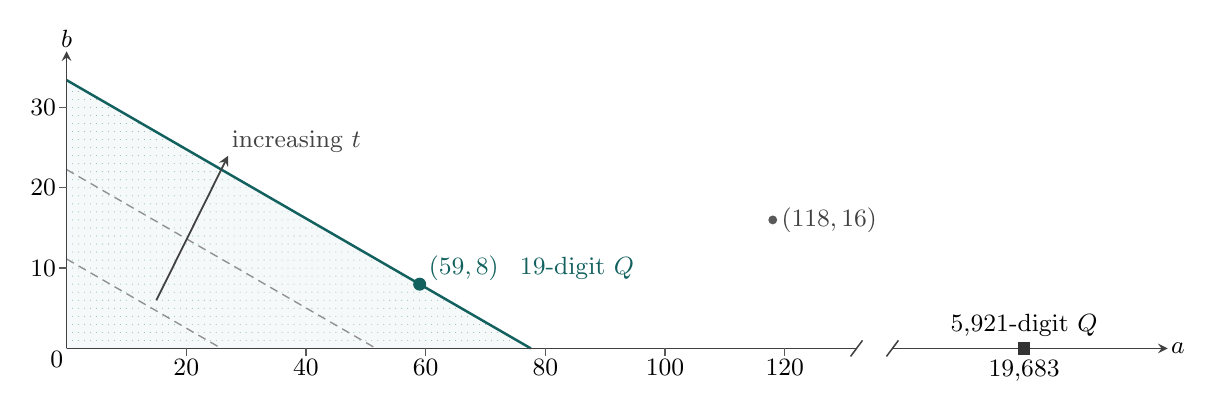
\begin{tikzpicture}[
    x=.76mm, y=1.02mm, font=\small,
    axis/.style={draw=black!75, line width=.55pt},
    tick/.style={draw=black!65, line width=.45pt},
    every node/.style={inner sep=1pt},
    >=stealth
]
\definecolor{productTeal}{HTML}{12615F}
\pgfmathsetmacro{\costRatio}{ln(5)/ln(2)}
\pgfmathsetmacro{\aIntercept}{59+8*\costRatio}
\pgfmathsetmacro{\bIntercept}{59/\costRatio+8}

% The row b contains the integers 0 <= a <= 59 + (8-b) log_2(5).
\fill[productTeal!4] (0,0) -- (\aIntercept,0) -- (0,\bIntercept) -- cycle;
\foreach \b in {0,...,33}{
    \pgfmathtruncatemacro{\lastA}{floor(59+(8-\b)*\costRatio)}
    \path[fill=productTeal!46] \foreach \a in {0,...,\lastA}
        {(\a,\b) circle[radius=.19pt]};
}
\foreach \portion in {1/3,2/3}{
    \draw[black!43, densely dashed, line width=.5pt]
        (0,{\portion*\bIntercept}) -- ({\portion*\aIntercept},0);
}
\draw[productTeal, line width=.9pt] (0,\bIntercept) -- (\aIntercept,0);
\draw[->, black!74, line width=.65pt] (15,6) -- (27,24)
    node[above right] {increasing $t$};

% The axis is linear through a = 130. Only the isolated axis minimum
% is shown to the right of the break.
\draw[axis,->] (0,0) -- (0,37) node[above] {$b$};
\draw[axis] (0,0) -- (132,0);
\draw[axis,->] (138,0) -- (184,0) node[right] {$a$};
\draw[axis] (131,-1) -- (133,1) (137,-1) -- (139,1);
\node[below left] at (0,0) {$0$};
\foreach \a in {20,40,60,80,100,120}
    \draw[tick] (\a,0) -- ++(0,-.9) node[below] {$\a$};
\foreach \b in {10,20,30}
    \draw[tick] (0,\b) -- ++(-1.2,0) node[left] {$\b$};

\fill[productTeal] (59,8) circle[radius=2.35pt];
\node[above right, text=productTeal] at (60,8)
    {$(59,8)$ \enspace 19-digit $Q$};
\fill[black!65] (118,16) circle[radius=1.6pt];
\node[right=2pt, text=black!75] at (118,16) {$(118,16)$};

\node[rectangle, fill=black!80, inner sep=0pt, minimum size=4.4pt] at (160,0) {};
\node[above=3pt] at (160,0) {5,921-digit $Q$};
\node[below=3pt] at (160,0) {$19{,}683$};
\end{tikzpicture}
}
\caption{Minimizing $P Q=2^a5^b$ at the fixed convergent $P/q=2^{16}/3^{10}$.
The fine dots represent the $1{,}352$ pairs with $2^a5^b\le 2^{59}5^8$.
The large markers show nonzero solutions of $2^a5^b\equiv\pm1\pmod q$.
As $t$ increases, the line $a\log 2+b\log 5=t$ first reaches such a solution
at $(59,8)$. On $b=0$ the first positive solution has $a=19{,}683$, shown off scale.}
\label{fig:exponents}
\end{figure}

The same minimum product also exhibits two smooth transitions of one
continued fraction.
The prefix $[1;2,1,1]$ contains the consecutive convergents $4/3,7/5$.
Its cylinder is $(11/8,7/5)$. Inside it lies
$P/q=81920/59049=2^{14}5/3^{10}$.
Taking $Q=N/P=2^{45}5^7$ and $P'=(N+1)/q$ gives a second admissible
pair in the very same continued fraction. Indeed the finite prefix
\[
 [1;2,1,1,2,1,1,4,31,1,3,2,1,46550814906941]
\]
has precisely $P/q,P'/Q$ for its last two convergents. Every infinite
continuation therefore exhibits both pairs. For this fixed $P/q$ the
value of $Q$ is minimal, since any smaller successor would give a
smaller admissible product.

At $q=59{,}049$, the two numerators $65{,}536$ and $81{,}920$ thus attain the
same least product $N_q$. The second numerator is $25\%$ larger, so its next
denominator $Q=N_q/P$ is $20\%$ smaller. In Theorem~\ref{th:exact}(i) the
construction finds divisors with $P/(q\sup I)\to1$, giving the endpoint term
$-\log(q\sup I)$. Along the exact-product transitions of a fixed $\xi$ in
part~(ii), $P/q\to\xi$, so $Q\sim N_q/(q\xi)$.

\section*{Verification}
Two AI reviewers independently checked the proofs of
Theorems~\ref{th:scales}, \ref{th:transfer}, and~\ref{th:exact} in the
24 November 2026 working draft. A separate audit of the six-page version
of that date confirmed the proofs, reviewed the exposition, and supplied
the argument for Corollary~\ref{cor:support}.

At $q=3^{10}$ the audit checker independently found $N_q=2^{59}5^8$ using
a table of powers of $2$ modulo $q$ and checked all $1{,}352$ products
through $N_q$. It reproduced the $5{,}921$- and $19$-digit minima at $P=65{,}536$ and
recovered all fourteen partial quotients of the nested example by applying
the Euclidean algorithm to $P'/Q$. To reproduce the finite checks, run
these commands using Python~3 from the
\href{https://github.com/twinheterodox/smooth-neighboring-convergents}{project repository}
root or the source archive's \texttt{anc/} directory.
\begin{verbatim}
python3 checks/check_examples.py
python3 checks/check_parents.py
python3 checks/independent-checks.py
\end{verbatim}

\begin{thebibliography}{9}
\small\raggedright
\setlength{\itemsep}{1pt}
\bibitem{adiceam} F. Adiceam, A note on the Hausdorff dimension of some
liminf sets appearing in simultaneous Diophantine approximation,
\emph{Mathematika} \textbf{59} (2013), 56--64.
\href{https://arxiv.org/abs/1209.6500v1}{arXiv:1209.6500v1}.
\bibitem{bn} Y. Bugeaud and K. D. Nguyen, Some arithmetical properties of
convergents to algebraic numbers, \emph{Pacific J. Math.} \textbf{326}
(2023), 17--36. \href{https://doi.org/10.2140/pjm.2023.326.17}{doi:10.2140/pjm.2023.326.17}.
\bibitem{dw} B. M. M. de Weger, Approximation lattices of $p$-adic
numbers, \emph{J. Number Theory} \textbf{24} (1986), 70--88.
\href{https://doi.org/10.1016/0022-314X(86)90059-4}{doi:10.1016/0022-314X(86)90059-4}.
\bibitem{em} P. Erd\H{o}s and K. Mahler, Some arithmetical properties of
the convergents of a continued fraction, \emph{J. London Math. Soc.}
\textbf{14} (1939), 12--18.
\href{https://doi.org/10.1112/jlms/s1-14.1.12}{doi:10.1112/jlms/s1-14.1.12}.
\bibitem{lm} J. Lelis and D. Marques, On a problem of Erd\H{o}s and Mahler
concerning continued fractions, \emph{Bull. Aust. Math. Soc.}
\textbf{95} (2017), 183--186.
\href{https://doi.org/10.1017/S0004972716000770}{doi:10.1017/S0004972716000770}.
\bibitem{marques} D. Marques, A neighbouring-denominator variant of the
Erd\H{o}s--Mahler conjecture, \emph{Bull. Aust. Math. Soc.}, published online
2026. \href{https://doi.org/10.1017/S0004972726102214}{doi:10.1017/S0004972726102214}.
Theorem and page references use
\href{https://arxiv.org/abs/2608.26455v2}{arXiv:2608.26455v2}.
\bibitem{counter} D. Marques, A counterexample to the Erd\H{o}s--Mahler
conjecture, preprint, 2026. \href{https://arxiv.org/abs/2611.13604v1}{arXiv:2611.13604v1}.
\bibitem{yu} K. Yu, $P$-adic logarithmic forms and group varieties III,
\emph{Forum Math.} \textbf{19} (2007), 187--280.
\href{https://doi.org/10.1515/FORUM.2007.009}{doi:10.1515/FORUM.2007.009}.
\end{thebibliography}
\end{document}
